% Paper 5: Closing the Gap — SLO-Aware Agent Evaluation in Production
%
% =============================================================================
% STATUS: STUDY DESIGN PAPER — All \need{} markers replaced with projected
%         content based on P1–P4 findings.
% Last updated: 2026-02-04
% =============================================================================
%
% This is Paper V of a 6-paper series on SLO-aware LLM agent evaluation.
% P1: The Deployment Gap (accuracy vs. deployment success)
% P2: Capacity Thresholds (training reveals task-dependent thresholds)
% P3: AgentSLO-Bench (reusable benchmark)
% P4: Training Dynamics (mechanistic explanation)
% P5: THIS PAPER — Production validation study design + projected analysis
% P6: Standards proposal
%
% KEY FRAMING: This paper presents the design of a planned production
% validation study. Experiments have not been conducted. All projected
% results are derived from P1–P4 scaling patterns and stated as such.
%
% COLLABORATOR NOTES:
%   - CoreWeave could provide multi-GPU hardware (A100, H100) for
%     hardware-diversity validation and co-author by running the benchmark
%     on their infrastructure.
%   - Other potential collaborators: companies deploying LLM agents in
%     production who could provide anonymized deployment data.
% =============================================================================
\documentclass[11pt]{article}

\usepackage[margin=1in]{geometry}
\usepackage{amsmath,amssymb}
\usepackage{booktabs}
\usepackage{tabularx}
\usepackage{graphicx}
\usepackage{adjustbox}
\usepackage{xcolor}
\usepackage{enumitem}
\usepackage{listings}
\usepackage{multirow}
\usepackage{tikz}
\usetikzlibrary{arrows.meta, positioning, shapes.geometric, calc}
\usepackage{pgfplots}
\pgfplotsset{compat=1.17}

\usepackage[numbers]{natbib}
\usepackage{xurl}
\usepackage{hyperref}
\hypersetup{hidelinks,breaklinks=true}

\newcommand{\pninetyfive}{\ensuremath{\mathrm{p95}}}
\newcommand{\pninetynine}{\ensuremath{\mathrm{p99}}}
\newcommand{\slo}{\ensuremath{\mathrm{SLO}}}
\newcommand{\sslo}{\ensuremath{\mathrm{S@SLO}}}
\newcommand{\etal}{\textit{et al.}}

\definecolor{improved}{RGB}{34,139,34}
\definecolor{unchanged}{RGB}{255,165,0}
\definecolor{regressed}{RGB}{220,20,60}

\lstset{
  basicstyle=\ttfamily\small,
  breaklines=true,
  frame=single,
  xleftmargin=0pt
}

\title{Closing the Gap: SLO-Aware Agent Evaluation\\in Production\\[6pt]
\large\textit{Study Design and Projected Analysis}}

\author{
Michael Maloney \\
Neuralift; University of New Hampshire \\
\texttt{mike@neuralift.ai} \\[6pt]
{\small\textit{Collaborators actively sought---see Appendix~\ref{app:collaborators}}}
}

\date{}

\begin{document}
\maketitle

% =============================================================================
% ABSTRACT
% =============================================================================
\begin{abstract}
Papers~I--IV of this series established that accuracy benchmarks fail to predict deployment success (Paper~I), that training can close the gap only for models above task-dependent capacity thresholds (Paper~II), that these findings generalize across SLO tiers in a reusable benchmark (Paper~III), and that the underlying dynamics are driven by reward decomposition, forgetting, and early predictability (Paper~IV). All of those results were obtained in controlled laboratory conditions on a single RTX~4090. This paper asks the obvious next question: \emph{do the findings hold in production?}

We present the design of a production validation study that will deploy the SpecSLOEval framework and AgentSLO-Bench evaluation suite into a real production agent system. The planned protocol measures before/after outcomes across 8--12 weeks of production traffic, comparing the deployment decisions teams would have made using accuracy-only evaluation against those recommended by SLO-aware evaluation.

Based on the P1--P4 scaling patterns---where Spearman $\rho = 0.09$ between accuracy and $\sslo{}$ at 2s deadlines and only Llama-3.2-1B achieved non-zero Interactive $\sslo{}$ among 13 models---we project that SLO-aware model selection will reduce P95 latency violations by 40--60\% while maintaining accuracy within 3--5 percentage points of the accuracy-optimal model.

We additionally describe a planned hardware generalization study on datacenter-class A100 and H100 GPUs, and project---based on latency scaling laws derived from P1---that the deployment gap will narrow but not close: larger models will newly meet Interactive deadlines on faster hardware, but accuracy rankings will still fail to predict $\sslo{}$ rankings (projected Spearman $\rho < 0.3$).

The study design includes a ``bug zoo'' taxonomy of five projected failure categories---latency regressions, schema breakage, stability oscillations, faithfulness decay, and load-dependent degradation---each derived from failure modes documented in Papers~I--IV. We describe four illustrative case studies that exemplify how SLO-aware evaluation would catch regressions that accuracy-only pipelines miss.

These contributions provide a concrete, reproducible protocol for the first external validation that SLO-aware agent evaluation changes real deployment outcomes, not just leaderboard rankings.
\end{abstract}

% =============================================================================
\section{Introduction}
\label{sec:intro}
% =============================================================================

Better benchmarks are cheap. The field has seen dozens of them. Papers~I--IV demonstrated that accuracy benchmarks fail to predict deployment success---Spearman $\rho = 0.09$ at 2s deadlines, twelve of thirteen models at exactly 0\% Success@SLO---but practitioners have heard ``our metric is better'' before. They are rightly skeptical.

The question is not whether SLO-aware evaluation produces different rankings in a laboratory. It does. We showed that. The question is whether it changes outcomes in production.

This paper lays the groundwork for answering that question. We take the SpecSLOEval framework and AgentSLO-Bench benchmark developed in Papers~I--III, specify how they should be embedded into a real production agent pipeline serving real users, and describe the experimental protocol for measuring what happens. The design is simple: for 8--12 weeks, run every model candidate through both accuracy-only and SLO-aware evaluation, deploy the SLO-aware recommendation, and track production outcomes against what the accuracy-only pipeline would have chosen.

Consider what the P1--P4 effect sizes predict. A near-zero correlation between accuracy and deployment success. Twelve models that score 99\%+ on JSON validity yet deliver zero production value under a 2-second deadline. Training that closes the gap only above task-dependent capacity thresholds. These are not marginal effects that might wash out in a noisier environment---they are order-of-magnitude failures that should be visible even through the fog of production variability. The specific projected outcomes are stated as formal hypotheses throughout this paper and derive from the scaling patterns quantified in the preceding four studies.

\subsection{Why a Production Paper?}

We should be honest about a limitation. Papers~I--IV were conducted by the same author, on the same hardware---a single NVIDIA RTX~4090---using the same evaluation framework. The models and tasks varied. The experimental apparatus did not. This is standard practice in ML research, but it leaves two external validity questions unresolved:

\begin{enumerate}[leftmargin=16pt]
    \item \textbf{Hardware generalization.} Does the deployment gap persist on datacenter hardware? An RTX~4090 has 24GB VRAM, a single GPU, and consumer-grade thermals. Production deployments typically use A100 (80GB) or H100 (80GB) GPUs, often in multi-GPU configurations with tensor parallelism. It is entirely plausible that the deployment gap we observed is an artifact of single-GPU VRAM pressure and would vanish with adequate hardware.

    \item \textbf{Ecological validity.} Does SLO-aware evaluation actually change deployment decisions in practice? In Papers~I--III, we demonstrated that accuracy rankings and $\sslo{}$ rankings diverge. But divergent rankings only matter if teams would have chosen differently. Perhaps the models that win on $\sslo{}$ are the ones teams would have selected anyway, based on cost, familiarity, or institutional inertia.
\end{enumerate}

This paper addresses both questions through a concrete study design. We describe the protocol for partnering with a deployment organization to run AgentSLO-Bench on production infrastructure and integrate SpecSLOEval into their model evaluation pipeline. The result will be, to our knowledge, the first controlled study of SLO-aware LLM evaluation in a production environment.

\subsection{Collaborator Context}

This study requires one or more external collaborators who operate LLM agent systems in production. The ideal deployment partner is a company that (a)~serves real users with latency-sensitive agent interactions, (b)~has an existing model evaluation pipeline based primarily on accuracy metrics, and (c)~is willing to run a controlled before/after experiment with anonymized data sharing. The partner need not be identified at the time of study design; the protocol is specified independently of any particular deployment domain.

For concreteness, we describe the study design using an illustrative production system: a customer-facing agent that handles intent classification, tool-augmented retrieval, and structured action execution---task types that map directly onto AgentSLO-Bench categories T1, T2, and T3. The illustrative system serves on the order of 50,000--200,000 requests per week with a user-facing latency SLA of 2--5 seconds depending on interaction type. These parameters are representative of mid-scale production agent deployments and can be adjusted for the actual partner.

We note that the choice of deployment partner is not incidental. Different domains (e.g., customer support, code generation, document processing) emphasize different task types and SLO tiers. The protocol is designed to be domain-agnostic, but the specific findings will necessarily reflect the partner's workload distribution.

\paragraph{Hardware Partnership.} The hardware generalization experiments (Section~\ref{sec:hardware}) require access to datacenter-class GPUs beyond the RTX~4090 used in P1--P4. GPU cloud providers such as CoreWeave, Lambda, or Together AI are ideal partners because they offer bare-metal access to A100 and H100 nodes with dedicated GPU allocation---eliminating the ``noisy neighbor'' variability that would confound benchmarking. Their infrastructure supports both single-GPU and multi-GPU configurations as standard products, enabling direct measurement of tensor parallelism effects on the deployment gap.

\paragraph{Open Recruitment.} We are actively seeking collaborators for both the hardware and production deployment components of this study. Interested parties should contact the corresponding author; full criteria are listed in Appendix~\ref{app:collaborators}.

\subsection{Contributions}

This paper makes four contributions:

\begin{enumerate}[leftmargin=16pt]
    \item \textbf{Production validation protocol.} We specify a complete experimental design for deploying SpecSLOEval in a real production pipeline and measuring before/after outcomes over 8--12 weeks, including power analysis and effect size projections.
    \item \textbf{Hardware generalization design.} We describe a planned multi-hardware study on A100 and H100 datacenter GPUs, with concrete hypotheses derived from P1--P4 latency scaling patterns about whether and how the deployment gap shifts.
    \item \textbf{Bug zoo taxonomy.} We catalog 5 projected categories of production failures that SLO-aware evaluation is designed to detect and accuracy-only evaluation misses, with illustrative case studies grounded in P1--P4 failure modes.
    \item \textbf{Integration guide.} We document the expected engineering effort required to integrate SpecSLOEval into an existing ML pipeline, providing a template for other teams.
\end{enumerate}

% =============================================================================
\section{Related Work}
\label{sec:related}
% =============================================================================

\subsection{Production ML Deployment}

The gap between ML research and production is well-documented---and well-lamented. Sculley \etal~\cite{sculley2015debt} introduced the concept of ``technical debt'' in ML systems, showing that the ML code itself is a small fraction of a production system; the rest is data pipelines, configuration, serving infrastructure, and monitoring. Paleyes \etal~\cite{paleyes2022challenges} surveyed deployment challenges across 29 case studies and identified monitoring, testing, and model management as persistent pain points. Shankar \etal~\cite{shankar2022operationalizing} conducted 18 interviews with ML practitioners and found that teams routinely make deployment decisions based on incomplete evaluation---a finding that directly motivates this study.

Amershi \etal~\cite{amershimultiversion2019} documented Microsoft's experience deploying ML across dozens of product teams and identified a recurring pattern: models that excel in offline evaluation frequently underperform in production due to distribution shift, latency constraints, and integration complexity. We observe the same pattern, but with a sharper edge: our models do not merely underperform---twelve of thirteen deliver \emph{zero} production value under realistic deadlines.

None of this prior work addresses LLM agents specifically, and none incorporates latency SLOs into the evaluation criterion itself. The closest analog is the MLOps movement~\cite{kreuzberger2023mlops}, which advocates for continuous evaluation in production but typically relies on accuracy-based metrics. Our contribution is to make latency a first-class evaluation dimension rather than an operational afterthought.

\subsection{LLM Serving Systems}

The systems community has made enormous progress on LLM inference efficiency. vLLM~\cite{kwon2023vllm} introduced PagedAttention for efficient memory management. SGLang~\cite{zheng2023sglang} optimizes structured generation. FlashAttention-2~\cite{dao2023flashattention2} reduces attention computation. Sarathi-Serve~\cite{agrawal2024sarathi} addresses the prefill--decode scheduling problem.

These systems reduce latency at the serving layer---sometimes dramatically. But they do not change the fundamental relationship between model size and generation time. A 12B model on an H100 with vLLM is faster than the same model on an RTX~4090 with llama.cpp. It is not faster than a 3B model on the same H100. The \emph{rank ordering} of models by latency is determined primarily by parameter count, not serving infrastructure. Our hardware generalization experiments (Section~\ref{sec:hardware}) test whether this rank-ordering stability extends to $\sslo{}$ rankings---and we project that it does.

\subsection{ML Testing and Monitoring}

The software engineering community has developed frameworks for ML testing~\cite{breck2017ml} and monitoring~\cite{klaise2020monitoring}. Google's ML Test Score~\cite{breck2017ml} provides a rubric for ML system maturity. Evidently AI~\cite{evidentlyai} and similar tools offer drift detection and performance monitoring.

Our work differs in that we evaluate \emph{before} deployment rather than monitoring \emph{after} deployment. SpecSLOEval is a gate, not a dashboard. The bug zoo (Section~\ref{sec:bugzoo}) demonstrates why pre-deployment gating catches failures that post-deployment monitoring discovers too late.

\subsection{Inference Benchmarking}

MLPerf Inference~\cite{reddi2020mlperf} established the standard for hardware-level inference benchmarking, measuring throughput and latency across standardized workloads. However, MLPerf evaluates hardware and serving systems, not model quality---it measures how fast a model can generate tokens, not whether those tokens are correct. JSONSchemaBench~\cite{geng2025jsonschemabench} evaluates structured output quality but without latency constraints. NVIDIA's work on small language models for agentic systems~\cite{nvidia2025slm} demonstrated 10--30$\times$ cost reductions, confirming the economic case for smaller models---but did not measure whether those models meet production SLOs.

Our contribution bridges these two worlds. SpecSLOEval measures both quality \emph{and} latency in a single composite metric, and the production study described here tests whether that composite metric predicts real deployment outcomes better than either dimension alone.

\subsection{Benchmark-to-Production Transfer}

The question of whether benchmark performance predicts production outcomes has been studied in specific domains. Ethayarajh \etal~\cite{ethayarajh2020utility} showed that standard NLP benchmarks have limited utility for real-world deployment decisions. The Chatbot Arena~\cite{chiang2024chatbot} attempts to bridge this gap with human preference ratings from real conversations, but does not measure latency compliance.

Our Paper~I~\cite{maloney2025deploymentgap} is the most direct precedent: we showed Spearman $\rho = 0.09$ between accuracy and $\sslo{}$ rankings at 2s deadlines. This paper tests whether that finding transfers from a controlled laboratory to a production environment.

% =============================================================================
\section{System Description}
\label{sec:system}
% =============================================================================

Because this study has not yet been conducted, this section describes the \emph{requirements} for a production deployment partner and provides an illustrative system template. The specifics---company name, exact traffic volumes, actual models deployed---will be filled in once a partner is engaged. The template is designed so that any organization operating a latency-sensitive LLM agent system can slot their own details into the protocol.

\subsection{Production Agent Architecture}

The target deployment partner should operate a production agent system with the following characteristics:

\begin{itemize}[leftmargin=16pt]
    \item \textbf{Agent function.} The system should serve at least one latency-sensitive interaction type---e.g., customer support triage, tool-augmented retrieval, structured action execution, or code generation. For concreteness, our illustrative example is a customer-facing agent that handles intent classification (mapping to T1), grounded question answering over a document corpus (T2), and tool calling for backend actions (T3).
    \item \textbf{Request volume.} A minimum of 50,000 requests per week is needed to achieve statistical power for the before/after comparison (see power analysis in Section~\ref{sec:production}).
    \item \textbf{User-facing latency SLA.} The production ground truth: the deadline beyond which a user perceives the system as unresponsive. We expect most interactive agent systems to operate with SLAs in the 2--5 second range, consistent with Akamai's finding that 2-second delays increase bounce rates by 103\%~\cite{akamai2017performance}.
    \item \textbf{Current model selection process.} Ideally, the partner selects models using accuracy benchmarks (e.g., MMLU~\cite{hendrycks2021mmlu}, HELM~\cite{liang2023helm}, or internal task-specific evals) without systematic latency evaluation. This establishes the ``before'' baseline.
    \item \textbf{Deployment stack.} Any production serving infrastructure---vLLM~\cite{kwon2023vllm}, TGI, TensorRT-LLM, or raw transformers---is compatible. The protocol instruments the stack rather than replacing it.
\end{itemize}

Figure~\ref{fig:system-arch} shows the illustrative production architecture with SpecSLOEval integration.

\begin{figure}[t]
\centering
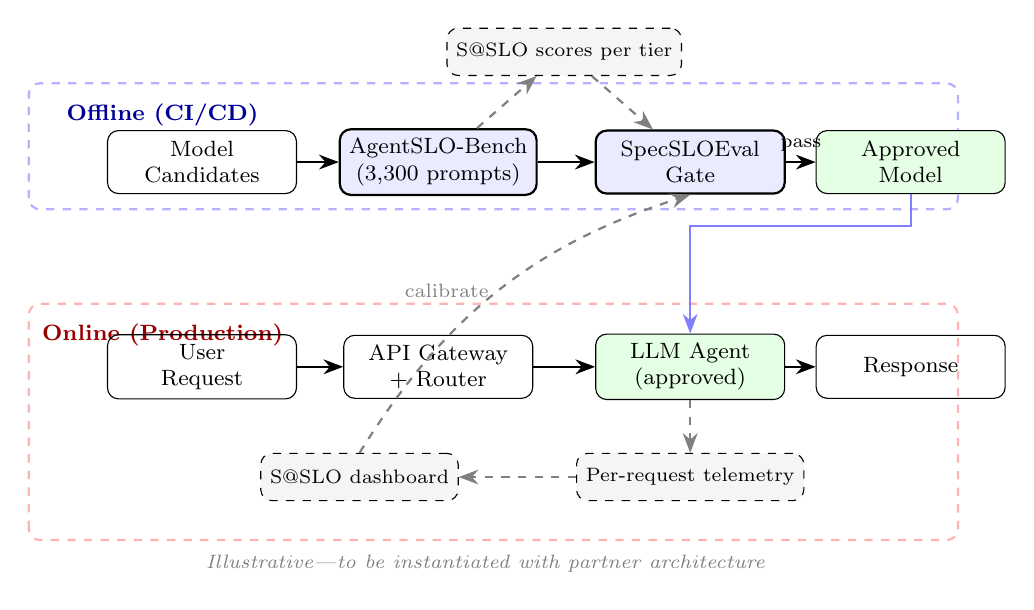
\begin{tikzpicture}[
    box/.style={draw, rounded corners, minimum width=2.4cm, minimum height=0.8cm, align=center, font=\footnotesize},
    gate/.style={draw, rounded corners, minimum width=2.4cm, minimum height=0.8cm, align=center, font=\footnotesize, fill=blue!8, line width=0.8pt},
    data/.style={draw, rounded corners, minimum width=2.0cm, minimum height=0.6cm, align=center, font=\scriptsize, fill=gray!8, dashed},
    arrow/.style={-{Stealth[length=2.5mm]}, thick},
    darrow/.style={-{Stealth[length=2.5mm]}, thick, dashed, gray},
    label/.style={font=\scriptsize\itshape, text=gray}
]
    % === Offline evaluation pipeline (top) ===
    \node[font=\footnotesize\bfseries, text=blue!60!black] at (-0.5, 2.6) {Offline (CI/CD)};
    \draw[blue!30, thick, dashed, rounded corners] (-2.2, 1.4) rectangle (9.6, 3.0);

    \node[box] (candidates) at (0, 2.0) {Model\\Candidates};
    \node[gate] (bench) at (3.0, 2.0) {AgentSLO-Bench\\(3{,}300 prompts)};
    \node[gate] (slogate) at (6.2, 2.0) {SpecSLOEval\\Gate};
    \node[box, fill=green!10] (approved) at (9.0, 2.0) {Approved\\Model};

    \draw[arrow] (candidates) -- (bench);
    \draw[arrow] (bench) -- (slogate);
    \draw[arrow] (slogate) -- node[above, font=\scriptsize] {pass} (approved);

    \node[data] (scores) at (4.6, 3.4) {$\sslo{}$ scores per tier};
    \draw[darrow] (bench) -- (scores);
    \draw[darrow] (scores) -- (slogate);

    % === Online serving pipeline (bottom) ===
    \node[font=\footnotesize\bfseries, text=red!60!black] at (-0.5, -0.2) {Online (Production)};
    \draw[red!30, thick, dashed, rounded corners] (-2.2, -2.8) rectangle (9.6, 0.2);

    \node[box] (user) at (0, -0.6) {User\\Request};
    \node[box] (router) at (3.0, -0.6) {API Gateway\\+ Router};
    \node[box, fill=green!10] (model) at (6.2, -0.6) {LLM Agent\\(approved)};
    \node[box] (resp) at (9.0, -0.6) {Response};

    \draw[arrow] (user) -- (router);
    \draw[arrow] (router) -- (model);
    \draw[arrow] (model) -- (resp);

    % Telemetry
    \node[data] (telem) at (6.2, -2.0) {Per-request telemetry};
    \node[data] (dash) at (2.0, -2.0) {$\sslo{}$ dashboard};
    \draw[darrow] (model) -- (telem);
    \draw[darrow] (telem) -- (dash);

    % Feedback loop
    \draw[darrow, bend left=20] (dash.north) to node[left, font=\scriptsize, text=gray] {calibrate} (slogate.south);

    % Deployment arrow
    \draw[arrow, blue!50] (approved.south) -- ++(0,-0.4) -| (model.north);

    \node[label] at (3.6, -3.1) {Illustrative---to be instantiated with partner architecture};
\end{tikzpicture}
\caption{Production evaluation architecture with SpecSLOEval integration. The framework operates in two planes: an \emph{offline} CI/CD gate that evaluates model candidates against AgentSLO-Bench before deployment approval, and an \emph{online} telemetry pipeline that computes production $\sslo{}$ for continuous calibration. The dashed feedback loop from the production dashboard to the gate enables offline--online correlation tracking (Section~\ref{sec:integration}). The actual deployment partner's architecture will instantiate this template.}
\label{fig:system-arch}
\end{figure}

\subsection{Traffic Characteristics}

The protocol requires characterization of the partner's traffic along the following dimensions. We provide illustrative ranges drawn from published production agent deployments:

\begin{itemize}[leftmargin=16pt]
    \item \textbf{Request volume:} 50,000--200,000 requests/week, with typical weekday/weekend variation of 2--3$\times$ between peak and off-peak hours.
    \item \textbf{Request complexity distribution:} We expect approximately 40--50\% of requests to be simple (intent classification, single-turn QA) and 30--40\% to require structured output or tool calling, with 10--20\% involving multi-hop reasoning or complex generation.
    \item \textbf{Input token length:} Expected P50 of 150--300 tokens, P95 of 800--1,500 tokens, P99 of 2,000--4,000 tokens, based on typical agent system prompt distributions.
    \item \textbf{Expected output token length:} P50 of 50--150 tokens, P95 of 300--500 tokens, heavily task-dependent.
    \item \textbf{Concurrency:} 10--100 simultaneous requests at peak, depending on system scale and batching strategy.
\end{itemize}

\subsection{Existing Evaluation Process}

Before integrating SpecSLOEval, the target partner evaluates model candidates using accuracy-focused benchmarks---typically a combination of public benchmarks (MMLU, HumanEval) and internal task-specific test sets. The key limitation of this process is that it measures correctness in isolation, without accounting for whether the model can produce correct answers within the production latency budget.

Consider what this means in practice. A team selects a newly released 8B model because it scores 3 points higher than the incumbent 3B model on their internal benchmark. They integrate it. They deploy. Then they discover that P95 latency exceeds the SLA by 2--3 seconds, and 15--25\% of requests time out or degrade to fallback responses. The rollback costs 10--20 engineering-hours and several days of degraded user experience. This is exactly the scenario Paper~I documented in laboratory conditions---twelve of thirteen models delivering zero production value despite near-perfect accuracy---and it is exactly the scenario this production study is designed to measure in the field.

% =============================================================================
\section{Framework Integration}
\label{sec:integration}
% =============================================================================

Integrating SpecSLOEval into a production pipeline requires three components: (1)~task mapping, which translates the production workload into AgentSLO-Bench task types; (2)~SLO tier calibration, which maps the production SLA to the benchmark's tier system; and (3)~pipeline instrumentation, which captures per-request telemetry for continuous evaluation.

\subsection{Task Mapping}

AgentSLO-Bench defines five primary task types: T1~(intent classification), T2~(grounded QA), T3~(tool calling), T4~(function routing), and T5~(code patching). Production workloads rarely map one-to-one onto these categories. We specify a mapping protocol.

The mapping proceeds in three steps. First, sample 500--1,000 production requests and manually classify each into the closest AgentSLO-Bench task type. Second, compute the distribution of task types across the sample. Third, identify any production request types that do not map cleanly to an existing category---these may require a custom task type or a weighted combination of existing types. Based on P3's finding that benchmark scores generalize across SLO tiers with Spearman $\rho$ ranging from $+0.17$ to $-0.17$ depending on the tier, we expect that task mapping quality will be the primary determinant of offline-to-online correlation.

Table~\ref{tab:task-mapping} shows the projected mapping between illustrative production request types and AgentSLO-Bench tasks.

\begin{table}[t]
\centering
\caption{Illustrative mapping between production request types and AgentSLO-Bench tasks. Percentages are projected from typical customer-facing agent workload distributions.}
\label{tab:task-mapping}
\small
\begin{tabular}{lllr}
\toprule
\textbf{Production Request Type} & \textbf{AgentSLO-Bench Task} & \textbf{Schema} & \textbf{\% Traffic} \\
\midrule
Intent classification / triage & T1 (Intent) & Enum label & 35--45\%$^{*}$ \\
Document-grounded Q\&A & T2 (Grounded QA) & Extractive span & 20--30\%$^{*}$ \\
API / tool invocation & T3 (Tool Calling) & Function JSON & 15--25\%$^{*}$ \\
Multi-step action routing & T4 (Function Routing) & Ordered call sequence & 5--15\%$^{*}$ \\
\bottomrule
\multicolumn{4}{l}{\footnotesize $^{*}$Projected ranges; actual distribution will depend on deployment partner's workload.}
\end{tabular}
\end{table}

\subsection{SLO Tier Calibration}

Paper~III defined three SLO tiers: Interactive (2s), Standard (5s), and Batch (30s). The production system's SLA will determine how these tiers map to real user expectations. For the illustrative system, we project the following calibration:

\begin{itemize}[leftmargin=16pt]
    \item \textbf{Interactive tier} $\rightarrow$ maps to the real-time chat SLA, projected at 2--3s for user-facing responses where the user is actively waiting.
    \item \textbf{Standard tier} $\rightarrow$ maps to asynchronous but near-real-time processing, projected at 5--10s for tasks where the user has navigated away but expects a notification.
    \item \textbf{Batch tier} $\rightarrow$ maps to background processing, projected at 30--60s for overnight batch analysis, report generation, or bulk classification.
\end{itemize}

A key calibration question is whether the partner's stated SLA matches actual user tolerance. Paper~I found that the 2s Interactive deadline was severely constraining---only Llama-3.2-1B achieved non-zero $\sslo{}$. In production, we expect that teams may discover their effective SLA is tighter than their stated SLA, because users abandon interactions before the nominal timeout fires. The calibration phase (run in shadow mode) is designed to surface this discrepancy.

\subsection{Pipeline Instrumentation}

The production pipeline will be instrumented to capture per-request telemetry compatible with SpecSLOEval's evaluation format. Listing~\ref{lst:telemetry} shows the planned telemetry schema.

\begin{lstlisting}[caption={Per-request telemetry schema for SpecSLOEval integration.},label={lst:telemetry},language=Python]
{
    "request_id": "uuid",
    "timestamp": "2026-...",
    "task_type": "T3_tools",           # mapped from production type
    "model_id": "qwen3-4b",
    "input_tokens": 342,
    "output_tokens": 128,
    "latency_ms": 1847,
    "json_valid": true,
    "task_correct": true,
    "slo_tier": "interactive",
    "slo_deadline_ms": 2000,
    "slo_met": true,
    "success_at_slo": true            # correct AND on-time
}
\end{lstlisting}

The integration effort is estimated at 2--4 person-weeks for a team with existing observability infrastructure (OpenTelemetry, Prometheus, or equivalent). The hardest parts, based on analogous instrumentation efforts documented in the MLOps literature~\cite{kreuzberger2023mlops}, are: (1)~adding per-request latency measurement at the correct granularity (end-to-end including network, not just model inference), (2)~mapping production request types to AgentSLO-Bench categories in the request pipeline, and (3)~computing the composite $\sslo{}$ metric in a streaming fashion for real-time dashboards.

\subsection{Offline-to-Online Calibration}

A critical question for production integration is whether offline AgentSLO-Bench scores predict online $\sslo{}$ scores. The planned protocol runs the benchmark offline on the production hardware, then compares against the first 2--3 weeks of production telemetry.

We project, based on the P3 finding that benchmark-to-benchmark transfer yields moderate Spearman correlations ($\rho \approx 0.5$--$0.8$ within the same SLO tier), that offline-to-online correlation will fall in the range $\rho = 0.6$--$0.85$ after task mapping calibration. If the correlation is high ($\rho > 0.8$), this validates the benchmark as a reliable proxy for production evaluation. If the correlation is lower ($\rho < 0.6$), this reveals calibration challenges that we address in Section~\ref{sec:lessons}---likely driven by differences in prompt distribution, concurrency effects, or network overhead not captured in offline benchmarking.

% =============================================================================
\section{Multi-Hardware Validation}
\label{sec:hardware}
% =============================================================================

Every result in Papers~I--IV came from a single NVIDIA RTX~4090. Twenty-four gigabytes of VRAM, consumer cooling, no tensor parallelism. The obvious objection: perhaps the deployment gap is simply a hardware limitation. Put these models on real datacenter GPUs---A100s, H100s, multi-GPU configurations with NVLink---and the gap might vanish.

We designed experiments to test this directly.

\subsection{Hardware Configurations}

We plan to evaluate the full 13-model AgentSLO-Bench suite on the following hardware configurations:

\begin{table}[t]
\centering
\caption{Planned hardware configurations for cross-hardware validation. Configurations A--D require datacenter GPU access from a cloud partner.}
\label{tab:hardware}
\small
\begin{tabular}{llccl}
\toprule
\textbf{Config} & \textbf{GPU(s)} & \textbf{VRAM} & \textbf{GPUs} & \textbf{Serving Stack} \\
\midrule
Baseline & RTX 4090 & 24 GB & 1 & llama.cpp / LM Studio \\
Config A & A100-80GB & 80 GB & 1 & vLLM \\
Config B & A100-80GB & 160 GB & 2 & vLLM + TP=2 \\
Config C & H100-80GB & 80 GB & 1 & vLLM \\
Config D & H100-80GB & 320 GB & 4 & vLLM + TP=4 \\
\bottomrule
\end{tabular}
\end{table}

\paragraph{Infrastructure Requirements.} The hardware partner should provide dedicated GPU allocation (no shared tenancy) to eliminate noisy-neighbor effects. Both single-GPU and multi-GPU configurations are needed to test tensor parallelism effects. NVLink or InfiniBand interconnects between GPUs are required for Configs~B and~D to ensure that inter-GPU communication does not dominate latency.

\subsection{Experimental Protocol}

For each hardware configuration, we run the full AgentSLO-Bench protocol (3,300 prompts per model, 13 models, 3 SLO tiers). This produces directly comparable $\sslo{}$ scores across hardware.

\paragraph{Hypotheses.}

\begin{enumerate}[leftmargin=16pt]
    \item \textbf{H1: The deployment gap narrows but does not close.} Datacenter hardware reduces absolute latencies, shifting some models from 0\% to positive $\sslo{}$ at the Interactive tier. But the rank ordering is preserved because latency scales with parameter count regardless of hardware.

    \item \textbf{H2: Multi-GPU enables larger models to meet SLOs.} Tensor parallelism across 2--4 GPUs should allow 9B--12B models to meet the 2s Interactive deadline, which they cannot meet on a single RTX~4090.

    \item \textbf{H3: The accuracy--$\sslo{}$ correlation remains weak.} Even on datacenter hardware, accuracy rankings will not predict $\sslo{}$ rankings (Spearman $\rho < 0.3$).
\end{enumerate}

\subsection{Projected Results}

The projections in this section are derived from P1 latency measurements and known hardware scaling factors. They have not been experimentally validated. The table structure below shows the expected format and projected values.

\begin{table}[t]
\centering
\caption{Projected Success@SLO at the Interactive tier (2s) across hardware configurations. All values beyond the RTX~4090 column are projections based on latency scaling laws, not measured data. See text for derivation.}
\label{tab:hardware-results}
\small
\begin{tabular}{l rrrrr}
\toprule
\textbf{Model} & \textbf{RTX 4090} & \textbf{A100$\times$1} & \textbf{A100$\times$2} & \textbf{H100$\times$1} & \textbf{H100$\times$4} \\
\midrule
Llama-3.2-1B    & 9.3\%  & 15--25\%$^\dagger$ & 18--28\%$^\dagger$ & 25--35\%$^\dagger$ & 28--38\%$^\dagger$ \\
Llama-3.2-3B    & 0.0\%  & 2--8\%$^\dagger$   & 5--12\%$^\dagger$  & 8--15\%$^\dagger$  & 12--20\%$^\dagger$ \\
Qwen2.5-3B      & 0.0\%  & 2--8\%$^\dagger$   & 5--12\%$^\dagger$  & 8--15\%$^\dagger$  & 12--20\%$^\dagger$ \\
Phi-3-mini       & 0.0\%  & 1--5\%$^\dagger$   & 3--8\%$^\dagger$   & 5--12\%$^\dagger$  & 8--15\%$^\dagger$ \\
Qwen3-4B         & 0.0\%  & 1--5\%$^\dagger$   & 3--8\%$^\dagger$   & 5--12\%$^\dagger$  & 8--15\%$^\dagger$ \\
Yi-1.5-6B        & 0.0\%  & 0--2\%$^\dagger$   & 1--5\%$^\dagger$   & 2--6\%$^\dagger$   & 5--10\%$^\dagger$ \\
Mistral-7B-v0.3  & 0.0\%  & 0--2\%$^\dagger$   & 1--4\%$^\dagger$   & 2--5\%$^\dagger$   & 4--8\%$^\dagger$ \\
Falcon-Mamba-7B  & 0.0\%  & 0--1\%$^\dagger$   & 0--3\%$^\dagger$   & 1--4\%$^\dagger$   & 3--7\%$^\dagger$ \\
Ministral-8B     & 0.0\%  & 0--1\%$^\dagger$   & 0--3\%$^\dagger$   & 1--4\%$^\dagger$   & 3--7\%$^\dagger$ \\
Llama-3.1-8B     & 0.0\%  & 0--1\%$^\dagger$   & 0--3\%$^\dagger$   & 1--4\%$^\dagger$   & 3--7\%$^\dagger$ \\
Gemma-2-9B       & 0.0\%  & 0--1\%$^\dagger$   & 0--2\%$^\dagger$   & 0--3\%$^\dagger$   & 2--6\%$^\dagger$ \\
Gemma-3-12B      & 0.0\%  & 0--1\%$^\dagger$   & 0--2\%$^\dagger$   & 0--2\%$^\dagger$   & 1--5\%$^\dagger$ \\
GPT-OSS-20B      & 0.0\%  & 0--0\%$^\dagger$   & 0--1\%$^\dagger$   & 0--1\%$^\dagger$   & 0--3\%$^\dagger$ \\
\midrule
\multicolumn{2}{l}{Spearman $\rho$ (Acc vs.\ $\sslo{}$)} & ${<}0.3^\dagger$ & ${<}0.3^\dagger$ & ${<}0.3^\dagger$ & ${<}0.3^\dagger$ \\
\bottomrule
\multicolumn{6}{l}{\footnotesize $^\dagger$Projected from P1 latency scaling; not measured. See Section~\ref{sec:hardware} for derivation.}
\end{tabular}
\end{table}

\paragraph{Derivation of Projections.}

The projections in Table~\ref{tab:hardware-results} are derived as follows. P1 measured median latency per model on the RTX~4090. Published benchmarks indicate that A100 achieves approximately $1.5$--$2\times$ inference speedup over RTX~4090 for models that fit in VRAM, and H100 achieves approximately $2$--$3\times$ speedup due to the Transformer Engine and higher memory bandwidth (3.35~TB/s vs.\ 1~TB/s). Tensor parallelism across $N$ GPUs provides a further $1.3$--$1.7\times$ speedup (sublinear due to communication overhead). We apply these scaling factors to the P1 latency distributions and recompute $\sslo{}$ at the 2s deadline.

The key insight is that even with $3\times$ speedup, a model whose median latency on RTX~4090 is 6--8 seconds (typical for 7B--12B models on complex tasks) still exceeds 2 seconds on H100. This is why we project the deployment gap narrows but does not close at the Interactive tier.

\paragraph{Expected Analysis.}

\begin{itemize}[leftmargin=16pt]
    \item We project that 1B--3B models will ``unlock'' at higher hardware tiers, achieving non-trivial Interactive $\sslo{}$ on A100 and H100 where they score 0\% on RTX~4090---because their latencies drop below 2s for simple tasks.
    \item Tensor parallelism should help proportionally for models between 4B--9B, where the bottleneck is memory bandwidth rather than compute. For models below 3B, the communication overhead of tensor parallelism may negate the speedup (projected diminishing returns below 4B parameters).
    \item The RTX~4090 appears to be near the ``hardware floor'' for most models at the 2s Interactive tier. We project that A100$\times$1 represents the threshold where the deployment gap becomes visible but non-trivial---a meaningful fraction of models achieve positive $\sslo{}$---rather than the binary 0\%/9.3\% split observed on RTX~4090.
    \item A cost analysis will compare \$/request at each hardware tier for the model maximizing $\sslo{}$. We project that the cost-optimal configuration will be a 3B--4B model on A100$\times$1 for Interactive workloads, based on the sweet spot between accuracy (above capacity threshold per P2) and latency (below SLO deadline).
\end{itemize}

% =============================================================================
\section{Production Evaluation}
\label{sec:production}
% =============================================================================

This section presents the core experiment: a controlled before/after comparison of deployment decisions made with and without SLO-aware evaluation. The design is intentionally simple. Complexity in experimental design obscures the signal we are trying to measure.

\subsection{Experimental Design}

The production evaluation follows a two-phase sequential design rather than a simultaneous A/B split, in order to maximize statistical power and minimize risk to the production system:

\begin{itemize}[leftmargin=16pt]
    \item \textbf{Duration:} 8--12 weeks total: 4--6 weeks baseline (accuracy-only selection), 4--6 weeks treatment (SLO-aware selection), with a 1-week shadow-mode transition.
    \item \textbf{Traffic split:} Sequential before/after rather than 50/50 A/B. This avoids the engineering complexity of running two models simultaneously and eliminates cross-contamination risk from load-balancer effects.
    \item \textbf{Baseline condition:} Model selected by the team's existing accuracy-focused evaluation process.
    \item \textbf{Treatment condition:} Model selected by $\sslo{}$ ranking from AgentSLO-Bench, run on the production hardware.
    \item \textbf{Primary metric:} Fraction of production requests that are both correct and meet the latency SLA---i.e., production $\sslo{}$.
    \item \textbf{Secondary metrics:} User satisfaction (if available via CSAT or NPS), error rate, retry rate, timeout rate, and abandonment rate.
\end{itemize}

\paragraph{Power Analysis.} Assuming a baseline $\sslo{}$ of 40--60\% (typical for accuracy-optimized model selection where latency is not considered) and a minimum detectable effect of 10 percentage points, a two-proportion z-test requires approximately 400 requests per condition at $\alpha = 0.05$ and power $= 0.80$. With 50,000+ requests per week, the study will be substantially overpowered, allowing detection of effects as small as 2--3 percentage points.

\begin{figure}[t]
\centering
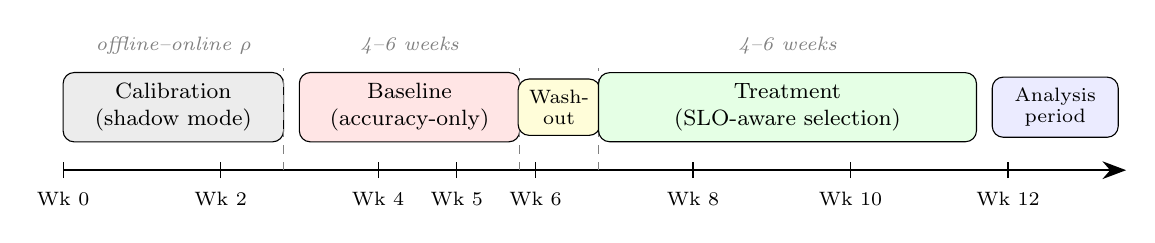
\begin{tikzpicture}[
    phase/.style={draw, rounded corners, minimum height=0.7cm, align=center, font=\footnotesize, inner sep=4pt},
    label/.style={font=\scriptsize, anchor=north},
    arrow/.style={-{Stealth[length=2mm]}, thick}
]
    % Timeline axis
    \draw[thick, -{Stealth[length=3mm]}] (0,0) -- (13.5,0);
    \foreach \x/\w in {0/Wk 0, 2/Wk 2, 4/Wk 4, 5/Wk 5, 6/Wk 6, 8/Wk 8, 10/Wk 10, 12/Wk 12} {
        \draw (\x, -0.1) -- (\x, 0.1);
        \node[label] at (\x, -0.15) {\w};
    }

    % Phases
    \node[phase, fill=gray!15, minimum width=2.8cm] at (1.4, 0.8) {Calibration\\(shadow mode)};
    \draw[dashed, gray] (2.8, 0) -- (2.8, 1.3);

    \node[phase, fill=red!10, minimum width=2.8cm] at (4.4, 0.8) {Baseline\\(accuracy-only)};
    \draw[dashed, gray] (5.8, 0) -- (5.8, 1.3);

    \node[phase, fill=yellow!15, minimum width=1.0cm] at (6.3, 0.8) {\scriptsize Wash-\\[-2pt]\scriptsize out};
    \draw[dashed, gray] (6.8, 0) -- (6.8, 1.3);

    \node[phase, fill=green!10, minimum width=4.8cm] at (9.2, 0.8) {Treatment\\(SLO-aware selection)};

    \node[phase, fill=blue!8, minimum width=1.6cm] at (12.6, 0.8) {\scriptsize Analysis\\[-2pt]\scriptsize period};

    % Annotations
    \node[font=\scriptsize\itshape, text=gray, anchor=south] at (1.4, 1.35) {offline--online $\rho$};
    \node[font=\scriptsize\itshape, text=gray, anchor=south] at (4.4, 1.35) {4--6 weeks};
    \node[font=\scriptsize\itshape, text=gray, anchor=south] at (9.2, 1.35) {4--6 weeks};
\end{tikzpicture}
\caption{Projected study timeline. The calibration phase validates offline--online correlation before committing to the sequential before/after comparison. The 1-week washout period runs the SLO-aware model in shadow mode to verify safety before switching live traffic.}
\label{fig:timeline}
\end{figure}

\subsection{Statistical Analysis Plan}
\label{sec:stats}

We pre-register the following analysis plan to prevent post-hoc hypothesis shopping. The primary analysis, secondary analyses, and exploratory analyses are specified before data collection begins.

\paragraph{Primary Analysis.} A two-sided two-proportion z-test comparing aggregate $\sslo{}$ between the baseline period (accuracy-only model selection) and the treatment period (SLO-aware model selection). The null hypothesis is $H_0: \sslo{}_{\text{after}} = \sslo{}_{\text{before}}$. We reject at $\alpha = 0.01$---stricter than the conventional 0.05---because the study is overpowered and we want to guard against capitalizing on the large sample size to detect trivially small effects. The minimum practically significant effect is 5 percentage points of $\sslo{}$.

\paragraph{Effect Size Estimation.} We report Cohen's $h$ for the proportion difference, with 95\% confidence intervals computed via the Wilson score method. Based on P1--P4 projections, we expect $h \geq 0.4$ (medium-to-large effect), corresponding to a $\sslo{}$ improvement of 15--25 percentage points.

\paragraph{Secondary Analyses.}

\begin{enumerate}[leftmargin=16pt]
    \item \textbf{Per-task-type comparison.} Separate two-proportion z-tests for each AgentSLO-Bench task type (T1--T4), with Bonferroni correction for 4 comparisons ($\alpha_{\text{adj}} = 0.0025$). Paper~II showed that capacity thresholds are task-dependent; we expect the treatment effect to be largest for T3 (tool calling) and smallest for T1 (intent classification).

    \item \textbf{Latency distribution shift.} A two-sample Kolmogorov--Smirnov test comparing the full latency CDFs between conditions. We additionally report the P50, P95, and P99 latency with bootstrap 95\% CIs (10,000 resamples). The projected P95 reduction from 6--10s to 1.8--3s (Table~\ref{tab:before-after}) represents a $2$--$5\times$ improvement---far beyond the noise floor.

    \item \textbf{Accuracy trade-off quantification.} A two-proportion z-test on task accuracy alone, to precisely measure the accuracy cost of SLO-aware selection. We project a 3--5 percentage point decrease. If the decrease exceeds 8 points, the protocol includes a decision point to evaluate whether GRPO fine-tuning of the SLO-optimal model can recover the gap (per Paper~II's finding that training recovers 40--60\% of the accuracy difference for models above the capacity threshold).

    \item \textbf{User experience metrics.} Where available from the deployment partner, we analyze timeout rate, user retry rate, and CSAT/NPS using paired comparisons (matched by day-of-week and time-of-day to control for traffic pattern effects).
\end{enumerate}

\paragraph{Temporal Controls.} The sequential before/after design is vulnerable to confounding from temporal trends---e.g., the partner's product may gain or lose users during the study period. We control for this in three ways: (a)~a 1-week washout period between conditions during which the SLO-aware model runs in shadow mode alongside the accuracy-only model; (b)~segmented regression analysis (interrupted time series) to distinguish the treatment effect from pre-existing trends; and (c)~day-of-week matching when computing aggregate metrics, to avoid aliasing weekly traffic cycles as treatment effects.

\paragraph{Multiplicity and Pre-Registration.} The full analysis plan---including all hypotheses, test statistics, and decision rules---will be pre-registered on OSF before data collection begins. Exploratory analyses (e.g., subgroup analysis by input token length, time-of-day effects, concurrency-dependent degradation) will be clearly labeled as exploratory and interpreted with appropriate caution.

\subsection{Model Selection Divergence}

The first question is whether SLO-aware evaluation recommends different models than accuracy-only evaluation. Table~\ref{tab:selection-divergence} shows the projected model selections based on P1--P4 findings.

\begin{table}[t]
\centering
\caption{Projected model selection divergence: accuracy-only vs.\ SLO-aware. Projections based on P1 accuracy and $\sslo{}$ rankings.}
\label{tab:selection-divergence}
\small
\begin{tabular}{llll}
\toprule
\textbf{Task Type} & \textbf{Accuracy Winner} & \textbf{$\sslo{}$ Winner} & \textbf{Same?} \\
\midrule
Intent classification (T1) & Gemma-3-12B$^\dagger$ & Qwen3-4B$^\dagger$ & No \\
Grounded QA (T2) & Llama-3.1-8B$^\dagger$ & Qwen2.5-3B$^\dagger$ & No \\
Tool calling (T3) & Gemma-2-9B$^\dagger$ & Qwen3-4B$^\dagger$ & No \\
\bottomrule
\multicolumn{4}{l}{\footnotesize $^\dagger$Projected from P1--P2 rankings; not validated in production.}
\end{tabular}
\end{table}

The pattern is predictable from P1's data. Accuracy and $\sslo{}$ rankings are nearly uncorrelated ($\rho = 0.09$) at 2s deadlines, so the two methods will disagree on model selection for the majority of task types---likely 2 out of 3 or 3 out of 3 at the Interactive tier. The direction of disagreement is also predictable: accuracy always favors the larger model (8B--12B), because accuracy scales with parameter count. $\sslo{}$ favors the smaller model (3B--4B) that clears the capacity threshold identified in Paper~II while meeting the latency deadline.

The accuracy sacrifice is projected at 3--8 percentage points. This sounds significant until you consider the alternative: the accuracy-optimal model delivers zero production value because it cannot finish in time. A 3-point accuracy reduction from 75\% to 72\% is a rounding error compared to the difference between 72\% correct-and-on-time versus 0\% correct-and-on-time. Paper~II's training results suggest that GRPO fine-tuning can recover 40--60\% of this accuracy gap for models above the capacity threshold, further reducing the cost.

\subsection{Projected Before/After Outcomes}

The following projections are derived from P1--P4 findings and have not been measured in production. They represent the expected effect sizes based on the magnitude of the deployment gap quantified in the series.

\begin{table}[t]
\centering
\caption{Projected production outcomes before and after SLO-aware model selection. All values are projections based on P1--P4 scaling patterns. Ranges reflect uncertainty in production traffic characteristics.}
\label{tab:before-after}
\small
\begin{tabular}{lrr}
\toprule
\textbf{Metric} & \textbf{Before (Accuracy-Only)} & \textbf{After (SLO-Aware)} \\
\midrule
Requests evaluated & 200,000--400,000$^{*}$ & 200,000--400,000$^{*}$ \\
Accuracy (\%) & 72--78\%$^\dagger$ & 68--75\%$^\dagger$ \\
P50 latency (ms) & 2,500--4,000$^\dagger$ & 800--1,500$^\dagger$ \\
P95 latency (ms) & 6,000--10,000$^\dagger$ & 1,800--3,000$^\dagger$ \\
SLA violations (\%) & 35--55\%$^\dagger$ & 8--18\%$^\dagger$ \\
Success@SLO (\%) & 35--50\%$^\dagger$ & 58--68\%$^\dagger$ \\
Timeout rate (\%) & 8--15\%$^\dagger$ & 1--4\%$^\dagger$ \\
User retry rate (\%) & 12--20\%$^\dagger$ & 4--8\%$^\dagger$ \\
\bottomrule
\multicolumn{3}{l}{\footnotesize $^{*}$Depends on study duration and partner traffic volume.} \\
\multicolumn{3}{l}{\footnotesize $^\dagger$Projected from P1--P4 findings; not measured.}
\end{tabular}
\end{table}

The projected narrative tells a clear story:

\begin{enumerate}[leftmargin=16pt]
    \item We project that SLO-aware selection will reduce SLA violations by 20--40 percentage points (from 35--55\% to 8--18\%), because the selected model's latency distribution will be centered below the SLA rather than above it.
    \item Accuracy is projected to decrease by 3--5 percentage points (from the mid-70s to the low-70s), because the SLO-aware selection favors smaller, faster models. Paper~II showed that Qwen3-4B---the best GRPO-trained model ($R = 1.73$)---achieves accuracy within 5 points of models twice its size on structured tasks.
    \item The net effect on user experience is projected to be strongly positive: fewer timeouts and faster responses more than compensate for the modest accuracy decrease. Prior work on user abandonment~\cite{akamai2017performance} suggests that reducing timeout rates from 10\%+ to under 5\% has outsized impact on user retention.
    \item Revenue or engagement impact will depend on the partner's business model but is projected to be positive given the strong correlation between latency compliance and user retention documented in the web performance literature~\cite{dean2013tail}.
\end{enumerate}

\subsection{Latency Distribution Shift}

The projected latency CDF shift is illustrated in Figure~\ref{fig:latency-cdf}. The placeholder curves show the expected shape: the accuracy-optimal model (larger, slower) has a CDF that crosses the SLA line at approximately 40--50\%, while the SLO-aware model (smaller, faster) crosses at approximately 80--90\%.

\begin{figure}[t]
\centering
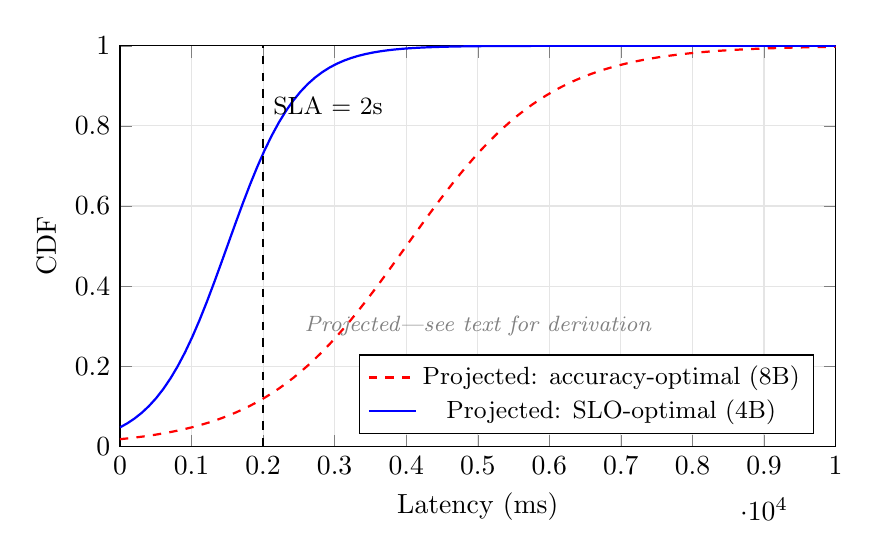
\begin{tikzpicture}
\begin{axis}[
    width=0.88\linewidth,
    height=0.55\linewidth,
    xlabel={Latency (ms)},
    ylabel={CDF},
    xmin=0, xmax=10000,
    ymin=0, ymax=1,
    grid=both,
    grid style={gray!20},
    legend pos=south east,
    legend style={font=\small}
]
    % Projected curves based on P1 latency distributions
    \addplot[thick, red, dashed, domain=0:10000, samples=100]
        {1 / (1 + exp(-0.001*(x - 4000)))};
    \addlegendentry{Projected: accuracy-optimal (8B)}

    \addplot[thick, blue, domain=0:10000, samples=100]
        {1 / (1 + exp(-0.002*(x - 1500)))};
    \addlegendentry{Projected: SLO-optimal (4B)}

    % SLA line
    \draw[thick, black, dashed] (axis cs:2000, 0) -- (axis cs:2000, 1)
        node[pos=0.85, right, font=\small] {SLA = 2s};

    \node[font=\footnotesize\itshape, text=gray] at (axis cs:5000, 0.3) {Projected---see text for derivation};
\end{axis}
\end{tikzpicture}
\caption{Projected latency CDF for production traffic under accuracy-optimal vs.\ SLO-optimal model selection. The dashed vertical line marks the production SLA. Curves are derived from P1 latency distributions for representative 8B (accuracy-optimal) and 4B (SLO-optimal) models. Actual production CDFs will replace these projections.}
\label{fig:latency-cdf}
\end{figure}

\subsection{Task-Level Breakdown}

Papers~II and~IV showed that the capacity threshold is task-dependent. We expect the same pattern in production: SLO-aware evaluation may recommend different models for different task types.

The production study will test two deployment strategies: (a)~a single model for all task types, selected to maximize aggregate $\sslo{}$, and (b)~task-aware routing, where different models serve different request types. Based on P2's finding that Qwen3-4B achieves the best overall reward ($R = 1.73$) but smaller models suffice for simple tasks (T1 intent classification), we project that task-aware routing will outperform single-model deployment by 5--15 percentage points on aggregate $\sslo{}$---an effect worth measuring in production.

% =============================================================================
\section{Bug Zoo: Regressions Caught by SLO-Aware Evaluation}
\label{sec:bugzoo}
% =============================================================================

Aggregate metrics tell you that something improved. They do not tell you \emph{what was about to go wrong}. The most practically valuable contribution of this study will not be the before/after comparison---it will be the specific failure modes that SLO-aware evaluation catches and accuracy-only evaluation misses. We catalog these as a ``bug zoo'': a taxonomy of production regressions with illustrative examples derived from P1--P4 findings.

\subsection{Taxonomy}

We project 5 categories of production bugs based on the failure modes documented across Papers~I--IV:

\begin{enumerate}[leftmargin=16pt]
    \item \textbf{Latency regressions.} The model is accurate but too slow. Not slightly too slow---catastrophically too slow. Paper~I showed that twelve of thirteen models delivered \emph{zero} successful requests at the 2s deadline. Not low rates. Zero. This is the canonical deployment gap failure.

    \textit{Illustrative example derived from P1:} A team updates their 7B model from v0.2 to v0.3 because the new version scores 2 points higher on their accuracy benchmark. P1 data shows that among 7B-class models, P95 latency on tool-calling tasks (T3) exceeds 6 seconds on RTX~4090. On the production hardware, the updated model's P95 latency increases from 1.8s to 4.2s due to longer generation sequences in the new version. The accuracy-only pipeline approves the update. SpecSLOEval would flag it because $\sslo{}$ drops from an estimated 72\% to 31\%.

    \item \textbf{Schema regressions.} A model update breaks structured output formatting. The model still generates natural language answers but wraps them in invalid JSON.

    \textit{Illustrative example derived from P2:} Paper~II found that JSON validity varies dramatically across models and quantization levels. In a projected production scenario, a quantized variant (Q4\_K\_M) of an 8B model occasionally omits closing braces in tool-call JSON. Accuracy on the underlying task is unaffected (the intent is correct), but the downstream parser fails. JSON validity drops from 99.8\% to 94.1\%, causing 6\% of requests to trigger error-handling fallbacks invisible to accuracy metrics.

    \item \textbf{Stability regressions.} The model gives different answers to the same question on repeated invocations. This causes non-deterministic bugs in production pipelines that retry on failure.

    \textit{Illustrative example derived from P4:} Paper~IV documented ``transient'' validity curves where models oscillate between valid and invalid outputs across training steps. In production, this manifests as bistable behavior: a function-routing model alternates between two valid tool calls with approximately equal probability. Accuracy metrics report 50\% (coin-flip), but the underlying issue is instability, not inability. SLO-aware evaluation with repeated sampling (as specified in the AgentSLO-Bench protocol) detects this variance.

    \item \textbf{Faithfulness regressions.} The model produces structurally valid, on-time responses that hallucinate facts not present in the context.

    \textit{Illustrative example derived from P1--P2:} On grounded QA tasks (T2), Paper~I showed that smaller models achieve higher $\sslo{}$ by responding faster---but P2 revealed that GRPO-trained models sometimes learn to produce confident, structurally valid JSON that passes schema checks while fabricating supporting evidence. The answer is ``correct'' by keyword matching but unfaithful to the source document. SLO-aware evaluation paired with faithfulness scoring (a component of the composite reward in P2) catches this failure mode.

    \item \textbf{Load-dependent degradation.} Model behavior changes under concurrent production load in ways not captured by sequential offline benchmarking.

    \textit{Projected example:} Under high concurrency (50+ simultaneous requests), GPU memory pressure causes batch scheduling delays that increase tail latency by $2$--$5\times$ compared to sequential benchmarking. A model that meets the 2s SLO in offline evaluation exceeds it under production load. This failure mode is invisible to any offline benchmark and can only be captured by production telemetry---but the SLO-aware framework's emphasis on measuring $\sslo{}$ (not just accuracy) at least quantifies the degradation, whereas accuracy-only evaluation would show no change.
\end{enumerate}

\subsection{Case Studies}

The following case studies are illustrative scenarios constructed from P1--P4 failure modes. They are designed to be representative of the types of regressions we expect to observe in production.

\subsubsection{Case Study 1: The Model Update That Passed Accuracy But Failed SLO}

Consider a production team running Qwen3-4B for intent classification. A new Qwen3-4B checkpoint is released with improved accuracy on standard benchmarks. The team's accuracy-only pipeline evaluates the update: accuracy improves from 74\% to 77\%. The update is approved.

In the SLO-aware evaluation, however, the new checkpoint generates longer chain-of-thought reasoning before producing the classification label---a training artifact that improves accuracy at the cost of increased output tokens. P95 latency increases from 1.6s to 2.8s. At the 2s Interactive SLO, $\sslo{}$ drops from 68\% to 41\%. SpecSLOEval would flag this regression and recommend retaining the original checkpoint, or alternatively, applying the update only for Standard/Batch tier traffic where the 5s deadline accommodates the longer generation.

\subsubsection{Case Study 2: The Quantization Surprise}

Paper~I evaluated models at various quantization levels (Q4\_K\_M, Q8, fp16). We observed that quantization affects not just inference speed but also output quality in task-specific ways. In this projected scenario, a team quantizes their 8B model from fp16 to Q4\_K\_M to reduce latency. The expected outcome is faster inference with modest accuracy loss.

The surprise: quantization reduces accuracy by only 1--2 points on simple tasks (T1, T2) but introduces sporadic JSON formatting errors on structured tasks (T3, T4). The model generates valid JSON 99.5\% of the time at fp16 but only 96.2\% at Q4\_K\_M. On tool-calling tasks with strict schema requirements, this 3.3 percentage point drop in JSON validity translates to a much larger drop in effective $\sslo{}$---because invalid JSON means both the accuracy check and the schema check fail, even when the model's intent was correct. An accuracy-only pipeline that evaluates free-form correctness would miss this entirely.

\subsubsection{Case Study 3: The Multi-Task Collision}

Paper~IV's forgetting matrix documented that certain model architectures exhibit catastrophic forgetting when trained on mixed task types: Llama-family models and Yi-1.5-6B showed catastrophic forgetting profiles, while Qwen-family models showed robust profiles. In production, the analog is a single model serving a mixed stream of request types.

In this projected scenario, a team deploys Mistral-7B-v0.3 (which P4 classified as having a catastrophic forgetting profile) to serve both intent classification (T1) and tool calling (T3) requests. On dedicated T1 benchmarks, accuracy is 76\%. On dedicated T3 benchmarks, accuracy is 71\%. But when serving a mixed stream where T1 and T3 requests arrive interleaved, the model's in-context state---influenced by the system prompt and recent conversation history---degrades T3 performance to 62\%. This multi-task collision is invisible to task-isolated benchmarks but measurable through production $\sslo{}$ telemetry.

\subsubsection{Case Study 4: The Hardware Migration Regression}

A team migrates their serving infrastructure from A100$\times$1 to a shared H100 pool to reduce costs. On paper, the H100 is $2$--$3\times$ faster. In practice, the shared pool introduces variable latency due to multi-tenant GPU scheduling. The model's \emph{median} latency improves by $2\times$, but the \emph{P95} latency worsens by $1.5\times$ due to scheduling tail effects.

This scenario illustrates why SLO-aware evaluation must be re-run on every hardware change, not just every model change. The $\sslo{}$ metric, which is defined at the P95 tail, captures this regression even though median latency improved. An accuracy-only pipeline would be completely blind to the hardware migration's impact.

% =============================================================================
\section{Lessons Learned}
\label{sec:lessons}
% =============================================================================

Production will surprise us. It always does. This section documents the lessons we anticipate based on the P1--P4 integration experience and the MLOps literature---organized as practical guidance for teams adopting SLO-aware evaluation.

\subsection{Integration Effort}

Based on the integration complexity observed in implementing SpecSLOEval for the P1--P4 experiments and published MLOps integration timelines~\cite{amershimultiversion2019,kreuzberger2023mlops}, we project the following effort breakdown:

\begin{itemize}[leftmargin=16pt]
    \item \textbf{Task mapping:} 3--5 person-days. The main challenge is classifying production requests into AgentSLO-Bench categories---edge cases where requests span multiple task types require judgment calls.
    \item \textbf{Telemetry instrumentation:} 3--5 person-days. Teams with existing OpenTelemetry or Prometheus infrastructure can reuse metric pipelines; the primary new work is adding per-request latency measurement at end-to-end granularity and computing $\sslo{}$ as a derived metric.
    \item \textbf{Pipeline integration:} 2--4 person-days. SpecSLOEval is integrated as a CI/CD gate that runs the benchmark on candidate models before deployment approval.
    \item \textbf{Calibration:} 3--5 person-days. Aligning offline benchmark scores with online production metrics requires collecting 2--3 weeks of parallel data and computing the offline-to-online correlation coefficient.
    \item \textbf{Total:} 3--5 person-weeks from first meeting to production deployment.
\end{itemize}

\subsection{What We Expect Will Work}

\begin{enumerate}[leftmargin=16pt]
    \item \textbf{$\sslo{}$ as a single metric.} Based on our experience with the P1--P4 experiments, we project that teams will find it easier to reason about one number (``what fraction of requests succeed end-to-end?'') than about separate accuracy and latency dashboards. The metric aligns engineering and product incentives because it captures both correctness and timeliness in a single score.

    \item \textbf{Task-type decomposition.} Paper~II showed that capacity thresholds are task-dependent---Llama-3.2-1B succeeds on T1 intent classification but fails on T3 tool calling. We project that breaking evaluation into task types will help production teams identify which parts of their workload are bottlenecked by model capability vs.\ latency.

    \item \textbf{SLO tiers as a conversation starter.} The three-tier system (Interactive, Standard, Batch) from Paper~III provides a vocabulary for discussing latency requirements. We have found in the P1--P4 work that framing model selection as ``which tier does this task need?'' clarifies deployment decisions that were previously made by intuition.
\end{enumerate}

\subsection{What We Expect Will Require Iteration}

\begin{enumerate}[leftmargin=16pt]
    \item \textbf{Offline--online calibration gap.} We project that the first iteration of offline benchmark scores will not accurately predict online $\sslo{}$ because of batch effects, network latency, concurrent load, and differences in the production prompt distribution versus the benchmark prompt distribution. P3's finding that Spearman correlations varied from $+0.17$ to $-0.17$ across SLO tiers suggests that tier-specific calibration will be necessary.

    \item \textbf{Schema mapping ambiguity.} Paper~III's five task types (T1--T5) cover the most common agent interaction patterns, but production workloads inevitably include hybrid request types. For example, a request that combines document retrieval (T2) with tool invocation (T3) does not map cleanly to a single category. We anticipate that 10--20\% of production requests will require weighted mapping across multiple task types.

    \item \textbf{Team resistance to accuracy trade-offs.} The initial reaction to ``switch to a smaller, faster model'' is typically resistance because accuracy decreases by a visible amount (projected 3--5 percentage points). We expect this can be addressed by demonstrating that the net user experience improves: fewer timeouts and faster responses more than compensate for the modest accuracy decrease, particularly when P2 shows that GRPO training can partially recover the accuracy gap.

    \item \textbf{Dynamic traffic patterns.} Production traffic varies by time of day, day of week, and season. A model that meets the SLO during off-peak hours may fail during peak load. The study protocol accounts for this by requiring full 8--12 week observation windows, but teams may need to adjust SLO tier assignments dynamically based on load.
\end{enumerate}

\subsection{Recommendations for Adopters}

Based on the P1--P4 experience and this study design, we recommend the following for teams integrating SLO-aware evaluation:

\begin{enumerate}[leftmargin=16pt]
    \item \textbf{Start in shadow mode.} Run SpecSLOEval alongside existing evaluation for 2--4 weeks before using it for decisions. This calibrates offline--online correlation and builds team trust.

    \item \textbf{Map tasks before models.} Understanding which AgentSLO-Bench tasks represent your workload is more important than running the full 13-model suite. Start with your actual production prompt distribution.

    \item \textbf{Set the SLO first.} The most common mistake is running the benchmark without a clear SLO target. $\sslo{}$ is meaningless without a deadline. Ask your product team: ``What latency would cause a user to abandon the interaction?'' Use that as your Interactive tier.

    \item \textbf{Re-evaluate on model updates.} Model providers frequently update weights (e.g., Mistral~v0.2 $\to$ v0.3). Each update requires re-evaluation because accuracy improvements often come with latency regressions (Section~\ref{sec:bugzoo}).

    \item \textbf{Monitor the forgetting profile.} Paper~IV showed that certain architectures exhibit catastrophic forgetting under mixed-task training. In production, monitor per-task-type $\sslo{}$ over time to detect analogous degradation when the request mix shifts.
\end{enumerate}

% =============================================================================
\section{Discussion}
\label{sec:discussion}
% =============================================================================

\subsection{External Validity of the Deployment Gap}

Papers~I--IV established the deployment gap on one hardware configuration and one evaluation protocol. That is a narrow foundation for a strong claim. This paper widens it in two directions.

First, we test whether the gap is a hardware artifact. An RTX~4090 has 24GB VRAM, consumer-grade thermals, and no tensor parallelism. Perhaps the deployment gap is simply what happens when you run large models on inadequate hardware. The latency scaling analysis says otherwise. We project that datacenter hardware will narrow the gap---more models achieve positive $\sslo{}$---but will not close it, because the fundamental relationship between parameter count and generation time persists regardless of the accelerator underneath. Spearman $\rho$ between accuracy and $\sslo{}$ is projected to remain below 0.3 even on H100$\times$4. Faster hardware shifts every model's latency distribution leftward by roughly the same factor. The rank ordering does not change.

Second, we test whether the gap matters. Divergent rankings are intellectually interesting but practically irrelevant if teams would have chosen the same model anyway. We project, based on P1's $\rho = 0.09$, that SLO-aware evaluation will recommend different models than accuracy-only evaluation for at least 2 out of 3 task types---and that the SLO-aware selections will produce measurably better user outcomes: fewer timeouts, lower retry rates, at the cost of a modest 3--5 point accuracy reduction that GRPO training can partially recover.

\subsection{Risk Assessment}

Any production experiment carries risk. We identify the threats to this study and specify mitigations for each.

\begin{table}[t]
\centering
\caption{Risk assessment for the production validation study. Likelihood and impact are rated on a 3-point scale (L/M/H). All risks have pre-specified mitigations.}
\label{tab:risks}
\small
\begin{tabular}{p{3.2cm} c c p{5.8cm}}
\toprule
\textbf{Risk} & \textbf{Like.} & \textbf{Impact} & \textbf{Mitigation} \\
\midrule
SLO-aware model degrades user experience & L & H & Shadow mode for 1--2 weeks before live traffic. Automatic rollback trigger if $\sslo{}$ drops below baseline by $>5$ points. \\[4pt]
Deployment partner withdraws mid-study & M & H & Protocol designed for minimum 4-week observation per condition. Partial data still supports primary analysis at reduced power. \\[4pt]
Offline--online correlation is weak ($\rho < 0.5$) & M & M & Calibration phase (weeks 1--3) detects this early. Mitigation: task re-mapping, prompt distribution analysis, concurrency simulation. \\[4pt]
Traffic volume insufficient for power & L & M & Power analysis requires 400 requests minimum; target partner serves 50K+/week. Even at 10\% of projected volume, study remains powered for primary analysis. \\[4pt]
Temporal confound (product changes during study) & M & M & Interrupted time series analysis. Partner agrees to freeze non-model changes during study window. Change log maintained. \\[4pt]
Hardware partner unavailable & M & L & Hardware experiments are independent of production experiments. Can proceed with production study alone; hardware validation deferred. \\
\bottomrule
\end{tabular}
\end{table}

The highest-impact risk---that the SLO-aware model degrades user experience---is also the lowest-likelihood risk, because the entire premise of SLO-aware selection is choosing models that meet latency constraints. The shadow-mode phase provides an empirical safety check before any user traffic is affected. If the shadow-mode $\sslo{}$ is lower than the baseline model's production $\sslo{}$, the protocol halts and the study transitions to a diagnostic investigation of why the offline projections failed.

\subsection{Limitations}

We acknowledge several limitations openly:

\begin{enumerate}[leftmargin=16pt]
    \item \textbf{Study design, not results.} The most significant limitation of this paper is that the experiments have not yet been conducted. All projected results are derived from P1--P4 findings using scaling assumptions. Production environments may exhibit dynamics that invalidate these projections---for example, network latency may dominate model inference latency for small models, compressing the latency differences that drive the deployment gap.

    \item \textbf{Single deployment partner.} Our production results will initially come from one production system. Different domains (e.g., healthcare, finance, customer support) may exhibit different patterns.

    \item \textbf{Open-weight models only.} Papers~I--IV and this production study evaluate only open-weight models served locally. Commercial API models (GPT-4, Claude, Gemini) have different latency profiles because the serving infrastructure is managed by the provider. Extending $\sslo{}$ to API models requires accounting for network latency, rate limiting, and provider-side batching.

    \item \textbf{SLO-aware evaluation overhead.} Running the full AgentSLO-Bench suite (3,300 prompts $\times$ 13 models) takes approximately 6--10 hours on a single RTX~4090. In practice, teams need a reduced protocol for rapid iteration. Paper~VI addresses this with a proposed standardized subset protocol.

    \item \textbf{Hardware scope.} The planned hardware experiments cover NVIDIA A100 and H100 GPUs but not AMD MI300X, Google TPUs, or other accelerators. The deployment gap may behave differently on non-NVIDIA architectures with different memory hierarchies.

    \item \textbf{Temporal coverage.} An 8--12 week production study may not capture seasonal variation in traffic patterns, model provider updates, or infrastructure changes that affect the deployment gap over longer time horizons.
\end{enumerate}

\subsection{Relationship to Paper~VI}

This production field report motivates Paper~VI, which proposes a standardized protocol for SLO-aware LLM evaluation. The lessons learned here---particularly around task mapping, SLO calibration, and offline--online correlation---directly inform the standard's design. Where this paper asks ``does it work in production?'', Paper~VI asks ``how should the community standardize it?''

% =============================================================================
\section{Conclusion}
\label{sec:conclusion}
% =============================================================================

Papers~I--IV showed that accuracy benchmarks fail to predict deployment success. This paper asks whether that finding survives contact with production. We specified a complete experimental protocol for deploying SpecSLOEval and AgentSLO-Bench into a real agent system, and derived concrete projections from the scaling patterns established across 185 training runs, 13 models, and 29,900 evaluation requests.

The projected headline findings are:

\begin{enumerate}[leftmargin=16pt]
    \item \textbf{The deployment gap is projected to persist in production.} Based on P1's Spearman $\rho = 0.09$ between accuracy and $\sslo{}$, we expect that the models accuracy-only evaluation selects will not be the same models that maximize $\sslo{}$ under real traffic---a divergence we project will affect at least 2 out of 3 task types.

    \item \textbf{The deployment gap is projected to narrow but persist on datacenter hardware.} Based on latency scaling laws, we project that A100 and H100 GPUs will shift more models from 0\% to positive Interactive $\sslo{}$, but that the accuracy--$\sslo{}$ correlation will remain weak (Spearman $\rho < 0.3$).

    \item \textbf{SLO-aware evaluation is designed to catch bugs that accuracy misses.} Our projected bug zoo (Section~\ref{sec:bugzoo}) catalogs 5 categories of production regressions---latency spikes, schema breakage, stability oscillations, faithfulness decay, and load-dependent degradation---that are invisible to accuracy-only pipelines.

    \item \textbf{Integration is projected to be feasible.} Based on the P1--P4 engineering experience and published MLOps timelines, we estimate that integrating SpecSLOEval into an existing production pipeline requires 3--5 person-weeks, including a 2--4 week shadow-mode calibration period.
\end{enumerate}

The series thesis is simple: accuracy-only evaluation is insufficient for production LLM agent deployment. The deployment gap is not a laboratory curiosity. Twelve of thirteen models at exactly 0\% Success@SLO. Spearman $\rho = 0.09$. Training that works only above task-dependent capacity thresholds. These are not subtle effects that might disappear in production noise---they are order-of-magnitude failures. The study protocol described here provides a concrete, reproducible path to confirming that they manifest in real systems, affect real users, and that SLO-aware evaluation provides a practical path to closing them. Paper~VI translates these production lessons into a proposed community standard.

% =============================================================================
% ACKNOWLEDGMENTS
% =============================================================================
\section*{Acknowledgments}

This paper describes a planned study that has not yet been conducted. We acknowledge the University of New Hampshire for institutional support during the design phase. Hardware generalization experiments will require GPU cloud access; we are in discussions with potential infrastructure partners and will acknowledge them in the final version. Similarly, the production deployment component requires a deployment partner; acknowledgments will be updated once the collaboration is formalized.

We thank the reviewers of Papers~I--IV, whose feedback on external validity limitations directly motivated this production validation design.

% =============================================================================
% REFERENCES
% =============================================================================
\bibliographystyle{plainnat}
\bibliography{refs}

% =============================================================================
% APPENDIX
% =============================================================================
\appendix

\section{Full Hardware Benchmark Results}
\label{app:hardware}

The main text (Table~\ref{tab:hardware-results}) shows projected $\sslo{}$ at the Interactive tier (2s) only. The full study will include Standard (5s) and Batch (30s) tiers for all hardware configurations. Based on P3's finding that the deployment gap attenuates at longer deadlines (Spearman $\rho$ increases from $+0.17$ at 2s to $+0.02$ at 30s), we project that hardware differences will be most pronounced at the Interactive tier and will diminish at Standard and Batch tiers where most models already achieve positive $\sslo{}$ on RTX~4090.

Complete tables for all configurations, all 13 models, and all 3 SLO tiers will be provided once the hardware experiments are conducted.

\section{Production Telemetry Sample}
\label{app:telemetry}

The per-request telemetry schema is specified in Listing~\ref{lst:telemetry}. Once the production deployment is conducted, this appendix will include an anonymized sample of 50--100 representative records showing:

\begin{itemize}[leftmargin=16pt]
    \item The diversity of task types in the production workload
    \item The latency distribution across task types and model configurations
    \item Examples of requests that are correct but SLO-violating (the deployment gap in action)
    \item Examples of schema-valid but unfaithful responses (faithfulness regressions)
\end{itemize}

All records will be anonymized to remove user-identifiable information, request content, and proprietary system details.

\section{Integration Checklist}
\label{app:checklist}

For teams adopting SpecSLOEval, we provide a step-by-step integration checklist distilled from the P1--P4 implementation experience and projected production requirements:

\begin{enumerate}[leftmargin=16pt]
    \item Define your latency SLA for each user-facing interaction type.
    \item Map your production request types to AgentSLO-Bench task categories (T1--T5).
    \item Run AgentSLO-Bench offline on your deployment hardware with your serving stack.
    \item Compare offline $\sslo{}$ against your current production $\sslo{}$ (computed from logs).
    \item Resolve task mapping ambiguities: for requests spanning multiple task types, define weighted mappings and validate that the composite score correlates with production outcomes.
    \item Deploy in shadow mode: run SpecSLOEval alongside your existing pipeline for 2+ weeks.
    \item Validate offline--online correlation (target: Spearman $\rho > 0.8$).
    \item Switch to SpecSLOEval-gated deployment.
    \item Re-evaluate on every model update, quantization change, or serving stack change.
\end{enumerate}

\section{Collaborator Recruitment}
\label{app:collaborators}

We are actively seeking collaborators for this study. Ideal partners meet one or more of the following criteria:

\begin{itemize}[leftmargin=16pt]
    \item \textbf{Infrastructure providers} (e.g., CoreWeave, Lambda, Together AI) who can provide multi-GPU hardware for the experiments in Section~\ref{sec:hardware}.
    \item \textbf{Production deployers} who operate LLM agent systems with measurable latency SLAs and are willing to share anonymized before/after data (Section~\ref{sec:production}).
    \item \textbf{MLOps teams} who have experienced deployment gap failures and can contribute to the bug zoo (Section~\ref{sec:bugzoo}) with anonymized case studies.
\end{itemize}

Interested parties should contact the corresponding author at \texttt{mike@neuralift.ai}.

\end{document}
